\chapter{Pion Analysis}

\subsection{Data Sample}

We decided to use only the data from the  -60 A, -100 A RunII configurations, because the beam composition for these 2 beamline configurations is available in G4Beamline. Run II data is better than Run I in terms of calorimetry and understanding of the detector. 

The used SamWeb definition is PionAna\_RunII\_60A\_100A\_lovely1\_elenag\_00  = 

Defined as ``defname: Lovely1 and data\_tier digits and lariat\_mid\_f\_mc7anb < 0 and create\_date < '2017-06-02' and run\_number != 9276 and run\_number != 9277 and run\_number != 8836 and run\_number != 9083 and run\_number != 9122 and run\_number != 8977 and run\_number != 8981 and run\_number != 8982 and run\_number != 8983 and run\_number != 8984 and run\_number != 8985 and run\_number != 8991 and run\_number != 8994 and run\_number != 8996 and run\_number >= 8767 and
run\_number <= 9635"

\begin{table}[]
\centering
\caption{My caption}
\label{my-label}
\begin{tabular}{|c|c|c|c|}
\hline
Stage                                          & -100A +64 GeV & -60A +64 GeV & Number of Evt \\
\hline
SamWebDefinition                     & 32.7\%        & 67.3\% & 3569206      \\
WCQuality                                  & 37.8\%        & 63.2\% &  553486      \\
P$_{WC4} > $ 420 MeV/c               & 50.8\%        & 49.2\% &  423294      \\
TOF Cut                                     & 32.7\%        & 67.3\% &       \\
\hline
                                               &               &             &\\
\hline
\end{tabular}
\end{table}

\subsection{Capture and Decay}
Our goal is to measure the total hadronic cross section for negative pions in argon. Since pion capture can be classified as an electromagnetic process and pion decay is a week process,  capture and decay represent unwanted interactions in our sample. We present here a study of capture and decay in Monte Carlo and the solution we adopted to mitigate their present in our sample. 

For this MC study, we use a sample of 359000 MC pions generated according to the beam profile with the DDMC described in \ref{sec:DDMC}. Unlike decay -- which may occur both in flight and at rest -- capture occurs predominantly
at rest. Thus, we can highly mitigate capture and decay at rest by removing pions whose energy is low enough to stop in the TPC. This translates into a momentum selection, where we keep only events whose WC momentum is above a certain threshold. 
Figure \ref{fig:CaptureMom} shows the true momentum distribution for the primary\footnote{We use here the Geant4 denomination "primary" to indicate that the pion considered does not undergo interactions modifying its energy before getting to the TPC. In fact, not every pion shot from wire chamber four will arrive to the TPC as primary,  some will decay or interact before the TPC, as explained in \textcolor{red}{reference to WC 2 TPC chapter}} pions that arrive to the TPC (pink), that capture (green) or decay (blue) inside the TPC, on a linear and log scale vertical axis. 

\begin{figure}[hpbt]
\centering
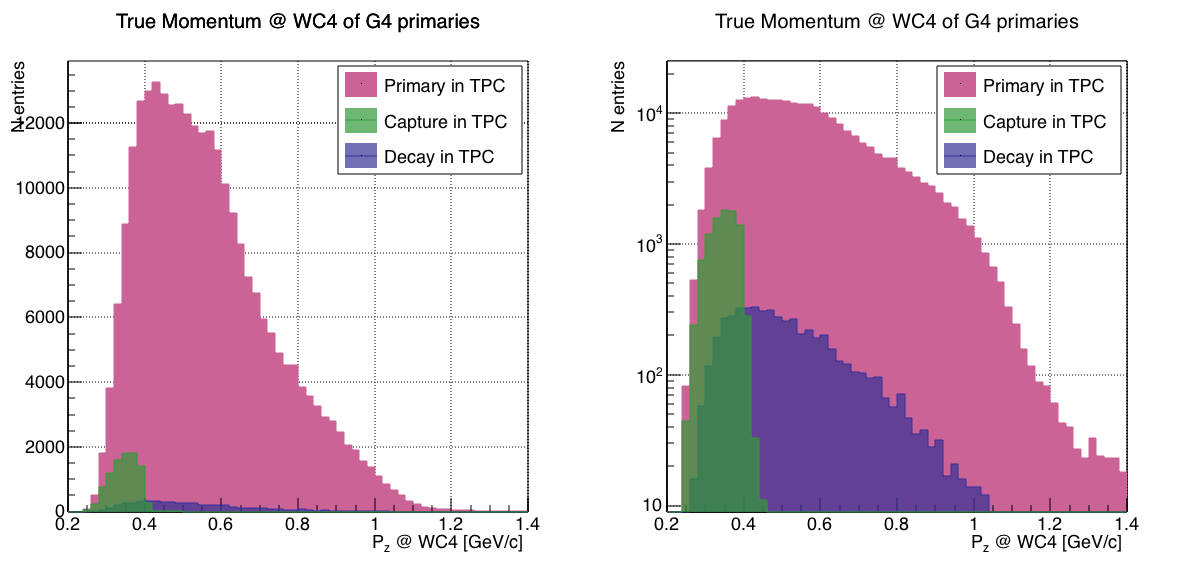
\includegraphics[width=15cm]{Chapters/C-PionImages/CDAsMomentumFunct.png}
\caption{True momentum distribution at wire chamber 4 for every simulated pion arriving in the TPC (pink), ending its life in capture (green) or in decay (blue) in the TPC, linear vertical axis on the left, logarithmic on the right. }
\label{fig:CaptureMom}
\end{figure}


In order to choose the selection value for the wire chamber momentum, it is beneficial to estimate the ratio of events which capture or decay that survive the selection in MC as a function of the momentum threshold, and compare it with the survival ratio for all events. This is done in figure \ref{fig:survRatio}. We define the survival ratio simply  as the number of events surviving the true momentum cut divided by the number of events of that given category. The survival ratio calculated separately for the three event categories explained above: total (pink), capture (green) and decay (blue).
Selecting pions with momentum greater than 420 MeV/c reduces the capture events by ~99\% while maintaining about 80\% of the total data sample. 
Figure \ref{fig:evtRatio} shows the ratio of events which end their life in capture (green) or decay (blue) over the total number of events as a as a function of the true momentum at wire chamber four. This ratio is slightly dependent on the inelastic cross section implemented in Geant4, as we are able to register a pion capture (or decay) only if it doesn't interact inelastically in the TPC. For momenta greater than 420 MeV/c, the percentage of capture events drops below 1\% and the percentage of decays is never above 2\%.

\begin{figure}[h!]
\centering
\begin{minipage}[t]{0.45\textwidth}
\centering
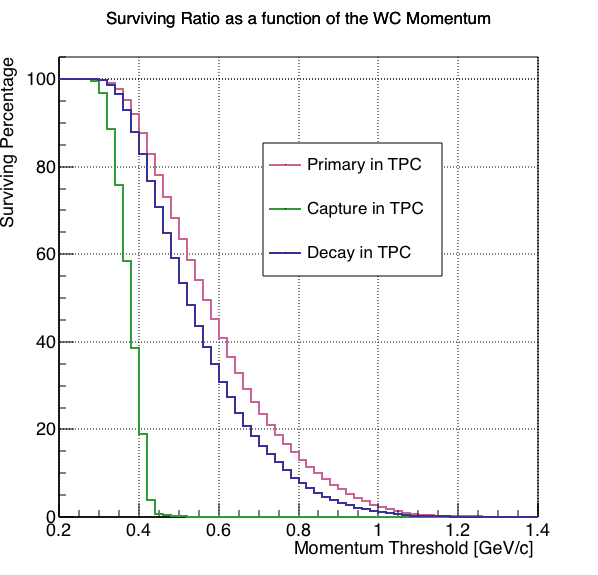
\includegraphics[width=7.5cm]{Chapters/C-PionImages/CDThreshold.png}
\caption{Survival ratio as a function of selection threshold on true momentum at wire chamber four for for every simulated pion arriving in the TPC (pink), capture (green) or in decay (blue).   }
\label{fig:survRatio}
\end{minipage}\hfill
\begin{minipage}[t]{0.45\textwidth}
\centering
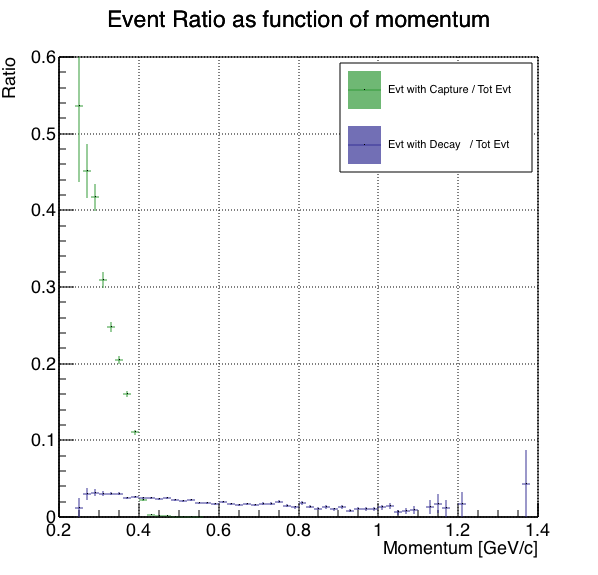
\includegraphics[width=7.5cm]{Chapters/C-PionImages/CDRatio.png}
\caption{Ratio between the capture (green) and decay (blue) events over the total number of events as a as a function of the true momentum at wire chamber four.}
\label{fig:evtRatio}
\end{minipage}
\end{figure}













